%%%%%%%%%%%%%%%%%%%%%%%%%%%%%%%%%%%%%%%%%
% baposter Portrait Poster
% LaTeX Template
% Version 1.0 (15/5/13)
%
% Created by:
% Brian Amberg (baposter@brian-amberg.de)
%
% This template has been downloaded from:
% http://www.LaTeXTemplates.com
%
% License:
% CC BY-NC-SA 3.0 (http://creativecommons.org/licenses/by-nc-sa/3.0/)
%
%%%%%%%%%%%%%%%%%%%%%%%%%%%%%%%%%%%%%%%%%

%----------------------------------------------------------------------------------------
%	PACKAGES AND OTHER DOCUMENT CONFIGURATIONS
%----------------------------------------------------------------------------------------

\documentclass[a0paper,portrait]{baposter}

\usepackage[font=small,labelfont=bf]{caption} % Required for specifying captions to tables and figures
\usepackage{booktabs} % Horizontal rules in tables
\usepackage{relsize} % Used for making text smaller in some places

\graphicspath{{figures/}} % Directory in which figures are stored

\definecolor{bordercol}{RGB}{40,40,40} % Border color of content boxes
\definecolor{headercol1}{RGB}{186,215,230} % Background color for the header in the content boxes (left side)
\definecolor{headercol2}{RGB}{80,80,80} % Background color for the header in the content boxes (right side)
\definecolor{headerfontcol}{RGB}{0,0,0} % Text color for the header text in the content boxes
\definecolor{boxcolor}{RGB}{186,215,230} % Background color for the content in the content boxes

\begin{document}

\background{ % Set the background to an image (background.pdf)
\begin{tikzpicture}[remember picture,overlay]
\draw (current page.north west)+(-2em,2em) node[anchor=north west]
{\includegraphics[height=1.1\textheight]{background}};
\end{tikzpicture}
}

\begin{poster}{
grid=false,
borderColor=bordercol, % Border color of content boxes
headerColorOne=headercol1, % Background color for the header in the content boxes (left side)
headerColorTwo=headercol2, % Background color for the header in the content boxes (right side)
headerFontColor=headerfontcol, % Text color for the header text in the content boxes
boxColorOne=boxcolor, % Background color for the content in the content boxes
headershape=roundedright, % Specify the rounded corner in the content box headers
headerfont=\Large\sf\bf, % Font modifiers for the text in the content box headers
textborder=rectangle,
background=user,
headerborder=open, % Change to closed for a line under the content box headers
boxshade=plain
}
{}
%
%----------------------------------------------------------------------------------------
%	TITLE AND AUTHOR NAME
%----------------------------------------------------------------------------------------
%
{\sf\bf Efficient segmentation algorithms for shark fin identification} % Poster title
{\vspace{1em} Author: L. Cilli\'{e}, 16010450 \hspace{0.5in} Project Advisors: Prof. B.M. Herbst, Dr. S.J. van der Walt \\ % Author names
{\vspace{0.5em} \smaller Honours Project, 2013, Applied Mathematics \\ Department of Mathematical Sciences, University of Stellenbosch}} % Author email addresses

\headerbox{Problem Statement}{name=Introduction,column=0,row=0}{
Identifying shark sightings is valuable for biological and ecological research --- such information can be used to predict migration
patterns, possible habitats and also in warning people about the
presence of sharks in a certain area.  Just as humans are identified by their fingerprints, sharks have an unique
dorsal fin structure.  In order to identify the sharks and to compare various shark sightings,
images of shark fins are analysed by a computer. 
This analysis consists of identifying the edges in the image and segmenting the
foreground, the shark, from the background, the sea.  
}

\headerbox{Data}{name=Data,column=0,below=Introduction}{
Below are a few examples from the database.  
The database consists of various shark fin images, taken on different dates and
at different locations.  
\begin{center}
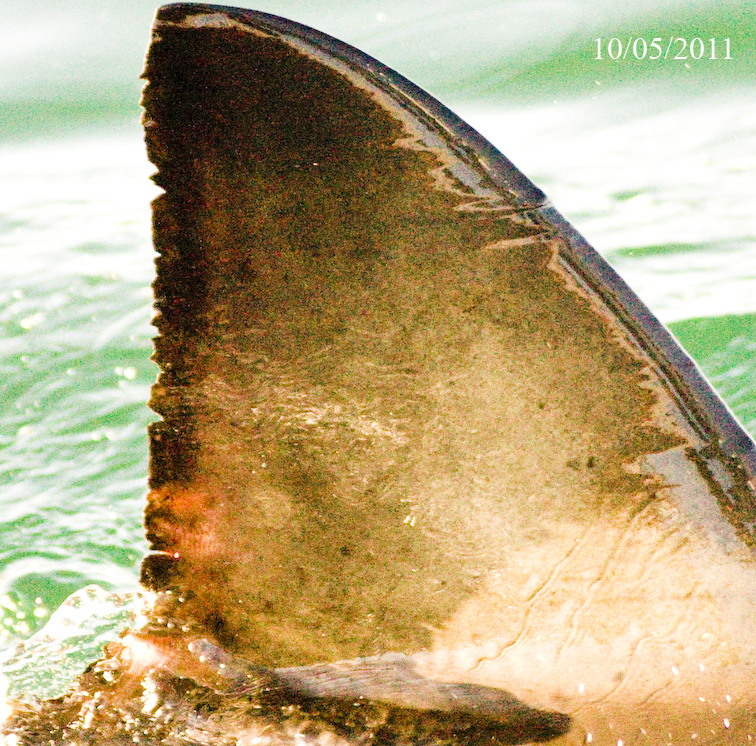
\includegraphics[width=0.49\linewidth]{haai1.jpg}
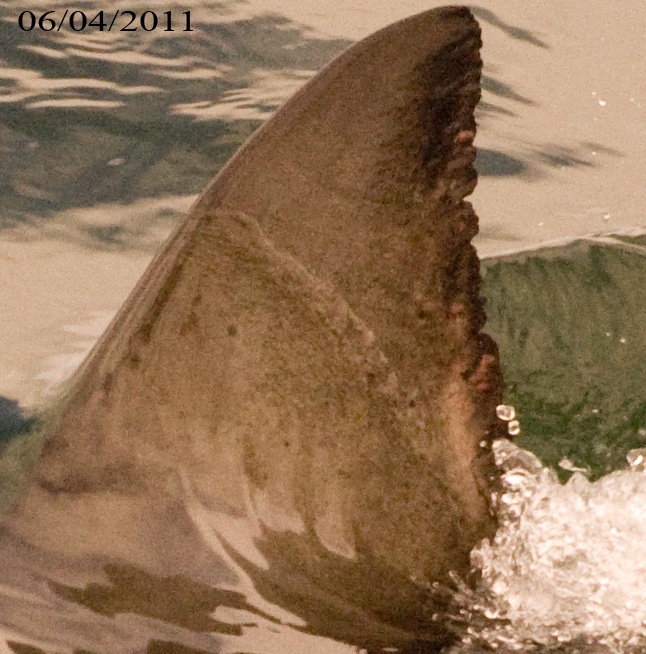
\includegraphics[width=0.49\linewidth]{haai4.jpg}
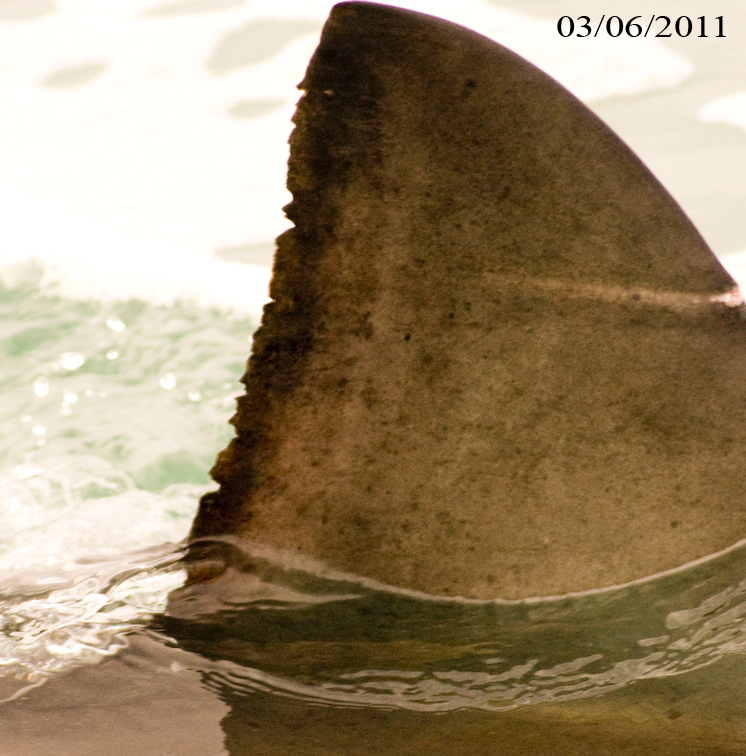
\includegraphics[width=0.49\linewidth]{haai2.jpg}
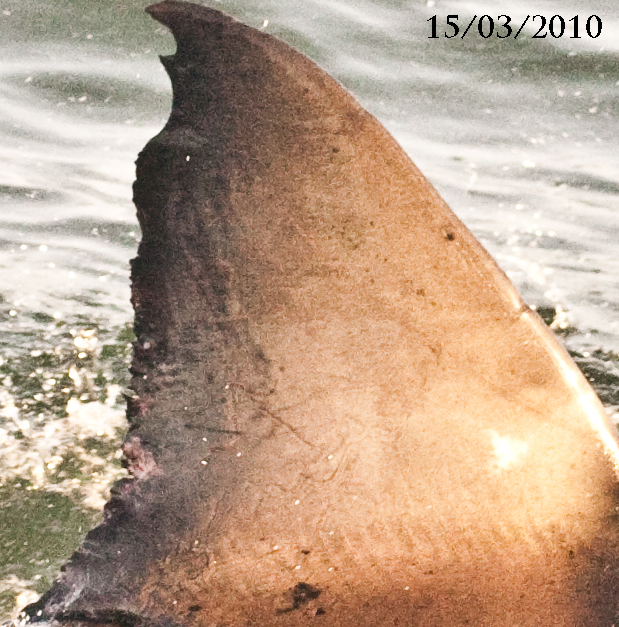
\includegraphics[width=0.49\linewidth]{haai5.jpg}
\captionof{figure}{Shark fin images.}
\end{center}

Although the images provided are of a good quality and have been cropped to only include the fin, the
foreground and background properties can still vary significantly, making segmentation a non-trivial problem.
}

\headerbox{Growcut}{name=Growcut,column=0,row=0, below=Data, above=bottom}{ % To reduce this block to 1 column width, remove 'span=2'
The Growcut algorithm is an interactive, multi-label segmentation algorithm
for N-dimensional images.  The algorithm is based on cellular automata, i.e.,
the user labels a few pixels, called the seed pixels, and the rest of the image is then segmented
automatically by a cellular automaton. \\

The Growcut algorithm takes the following parameters: an N-dimensional input image,
an initial state, which stores (foreground/background, strength) for
each pixel position or automaton.  The strength represents the
certainty of the state (e.g., 1 is a hard seed value that remains
constant throughout segmentation), the maximum number of automata iterations to allow   
(the segmentation may complete earlier if the state no longer varies) and the
size of the neighbourhood window.  The algorithm will return a segmented image, 
where a value of zero indicates background and a value of one indicates foreground. \\
}

\headerbox{Growcut continued}{name=Growcutc,column=1,row=0}{ % 
It is helpful to view the labelling process as ongoing growth and struggle of $K$ different species.
The species start to "grow" from the seeded pixels, trying to occupy the whole image.  
Each iteration involves every cell trying to "attack" its neighbour, cell $q$ "attacking" cell $p$ for instance. 
The strength of the attack is determined by the attacker's cell strength, $\theta_{q}$, and
the difference in intensity values of $p$ and $q$. \\

Whenever the attack strength is greater than the defend strength, the defending cell is "conquered" and
its strength and label is updated to that of the attacker. 
These iterations continue until either the maximum number of iterations is met or the automaton has converged,
where cell state seize to change.  Note that convergence is guaranteed since cell strength is increasing and bounded. \\

Here we show the result of the Growcut segmentation.
\begin{center}
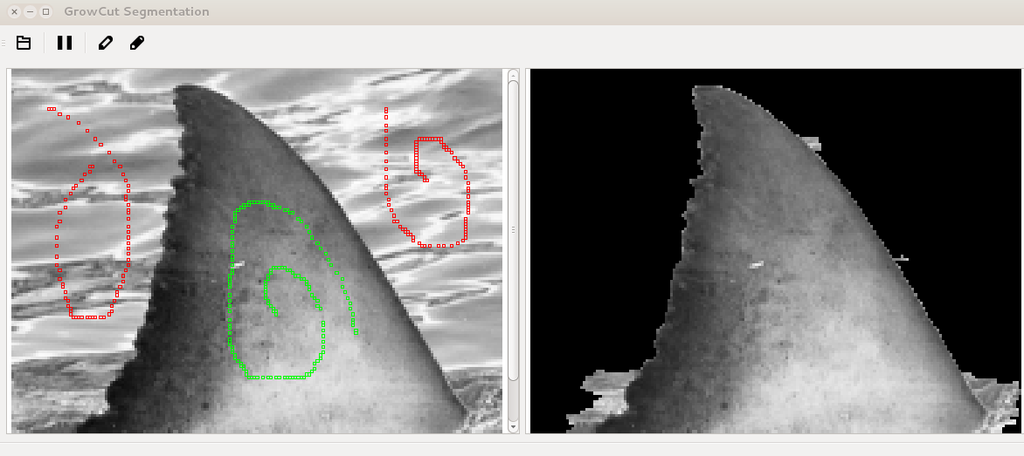
\includegraphics[width=1 \linewidth]{haaim}
\captionof{figure}{The Growcut algorithm.}
\end{center}
}

\headerbox{Pipeline}{name=Pipeline,column=1,row=0, below=Growcutc}{ % To reduce this block to 1 column width, remove 'span=2'
The procedure of identifying sharks can be
divided into several components, together forming an image processing pipeline, each implemented as part of
a bigger pipeline.  The first algorithm is an orientation detection
algorithm that will determine whether the shark fin is orientated to the left or the right in the image.
Then a segmentation algorithm will segment the shark fin from the image such that the path that defines the shark fin 
can easily be detected by the fin detection algorithm.  Thereafter a dynamic time warping algorithm is used
to compare the paths describing the fins and to see how shark fins in the database compare. \\

\begin{itemize}
 \item \textbf{ORIENTATION} To provide a consistent basis for further analysis, the orientation of the shark fin in the image is determined as the direction in which the shark is swimming.   The method of Principal Components Analysis (PCA) is used to determine the orientation of the shark fin.  When applying
PCA, we are interested in finding the direction of maximum variation in the data, the pixel values in the shark fin images.  Below is a dummy shark fin image where the orientation is detected using PCA.  Note the principal axis, largest eigenvector, in blue, which gives the orientation of the shark fin.
\begin{center}
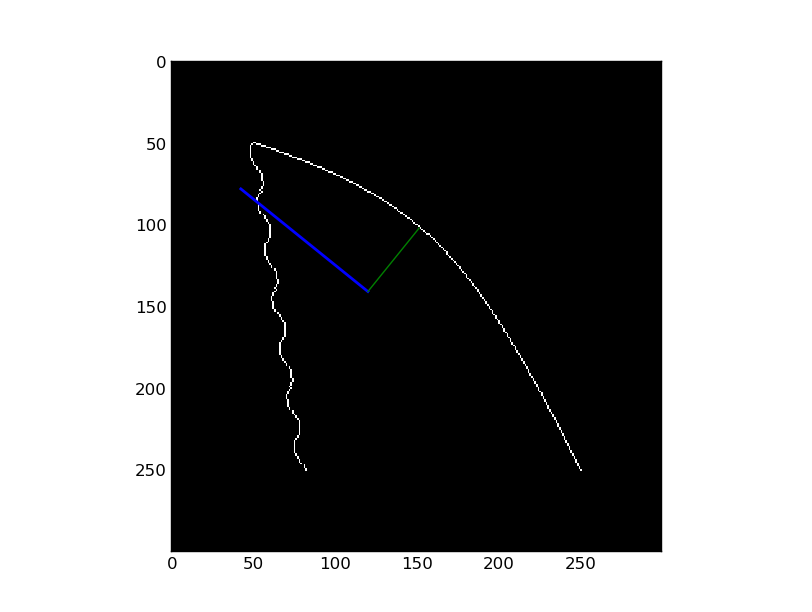
\includegraphics[width=0.5\linewidth]{orientation.jpg}
\captionof{figure}{Orientation of the shark fin detected by means of PCA.}
\end{center}

 \item \textbf{SEGMENTATION} .
 \item \textbf{FIN DETECTION} The objective is to identify the serrated part of the dorsal shark fin. In order
to do this, we need to extract this part of the fin, in such a way that it can be compared with other fins easily.
We use the Sobel operator to identify edges in the image.

In the figure below is an example of the path, in blue, that was detected on the shark
fin.
\begin{center}
 \centering
 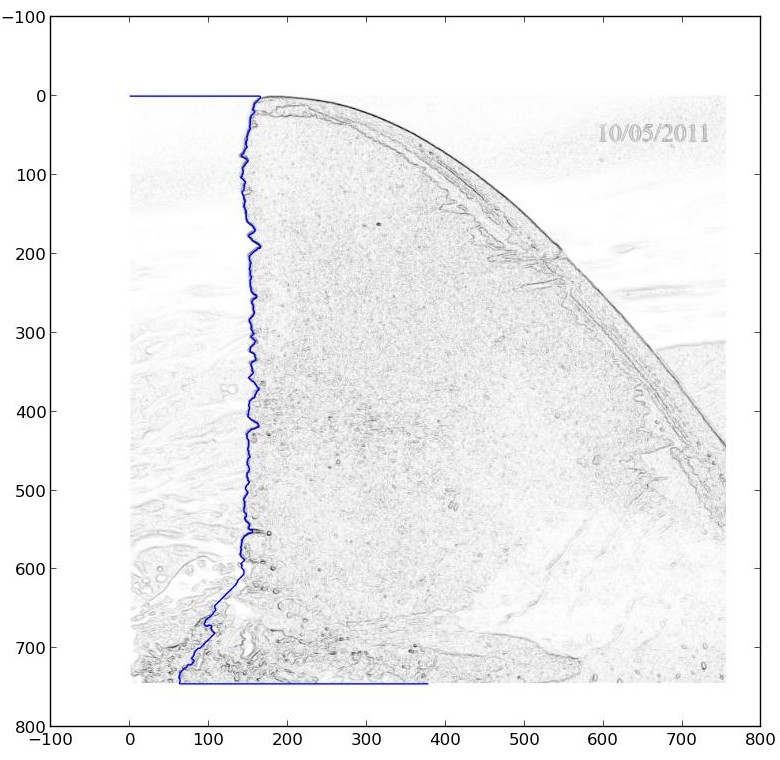
\includegraphics[width=0.5in]{path.jpg}
 \captionof{figure}{Fin path detected.}
\end{center}

 \item \textbf{FIN MATCHING} Dynamic time warping (DTW) is an algorithm used for
measuring the similarity between two similar sequences which may vary in time or speed.
\end{itemize}

}

\headerbox{Pipeline continued}{name=Pipelinec,column=2,row=0}{

}

\headerbox{Results}{name=Results,column=2,below=Pipelinec}{ % To reduce this block to 1 column width, remove 'span=2'
We show the path detected, in blue, on a few shark fin images.  Recall that only the top $\frac{2}{3}$ of the path is extracted, 
since the fins become more unreliable as we move closer to the body of the shark.  The images of the shark fins, shown below,
are a selection from which the fins were detected accurately. \\

\begin{center}
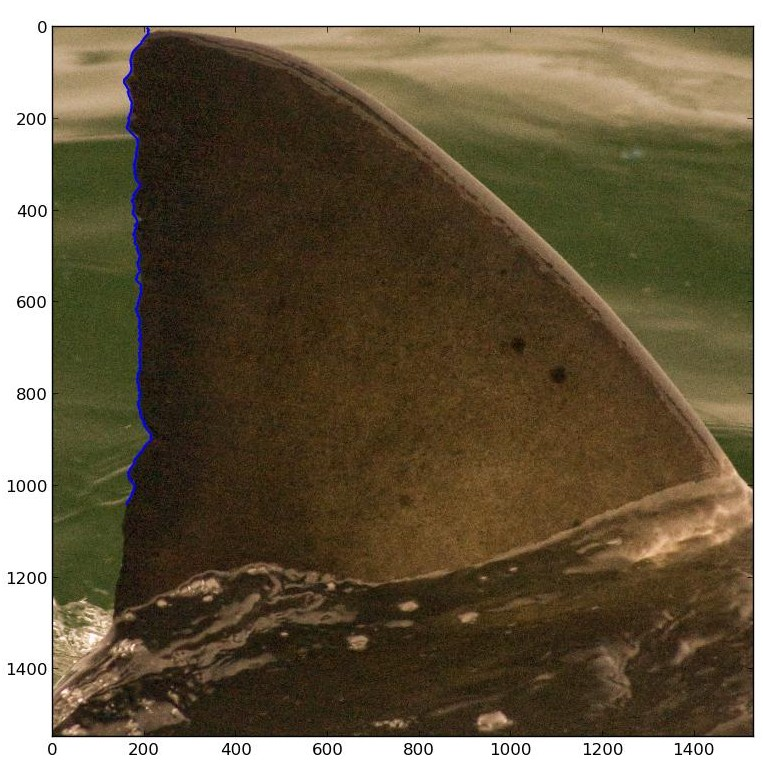
\includegraphics[width=0.49\linewidth]{findetect1.jpg}
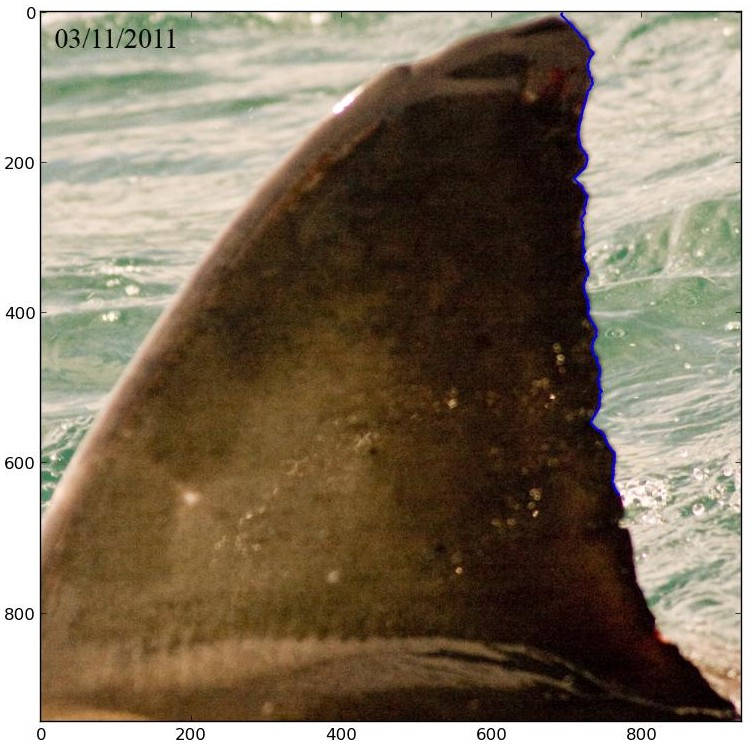
\includegraphics[width=0.49\linewidth]{findetect2.jpg}
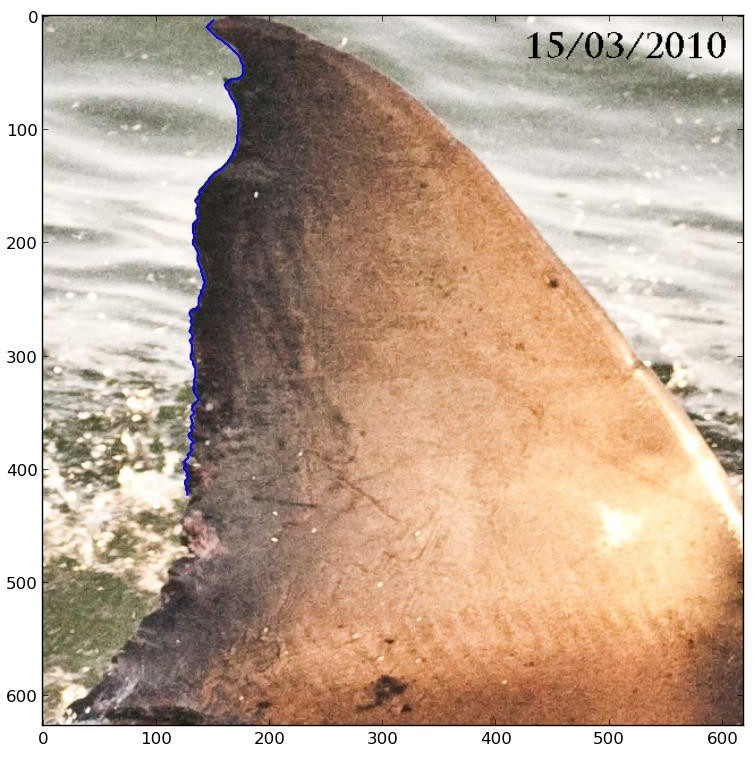
\includegraphics[width=0.49\linewidth]{findetect4.jpg}
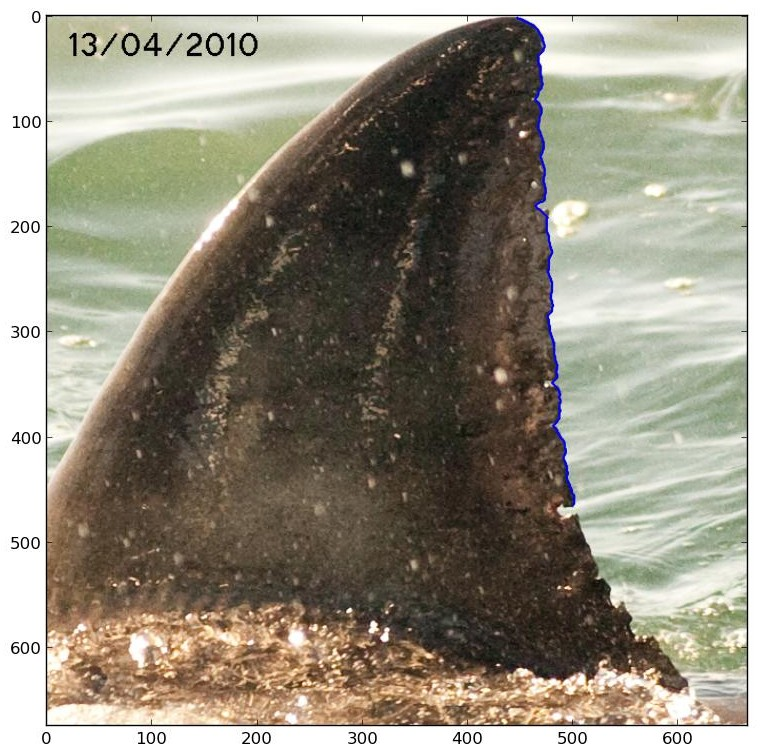
\includegraphics[width=0.49\linewidth]{findetect5.jpg}
\end{center}
}

\headerbox{Conclusion}{name=Conclusion,column=2,below=Results}{
This research project entails studying different segmentation algorithms with the aim of identifying sharks for various environmental and biological purposes.
The Growcut algorithm is discussed as the main segmentation algorithm.  Orientation detection, segmentation, fin detection and fin matching form the building blocks of an image processing pipeline.
}

\headerbox{Acknoweledgements}{name=Acknoweledgements,column=2,below=Conclusion}{
\smaller % Reduce the font size in this block
I am indebted to Ms. S. Andreotti for providing us with a sample from her carefully
curated set of photos used in this research project, 
Ms. T. Marais for her generous contribution to the development of the pipeline and 
Dr. N. Faggian for providing us with the Growcut gui.
}

\headerbox{References}{name=References,column=2,below=Acknoweledgements, above=bottom}{
\smaller % Reduce the font size in this block
\renewcommand{\section}[2]{\vskip 0.05em} % Get rid of the default "References" section title
\nocite{*} % Insert publications even if they are not cited in the poster

\bibliographystyle{unsrt}
\bibliography{sample} % Use sample.bib as the bibliography file
}

\end{poster}

\end{document}